El sistema Thary fue diseñado basandose en una organización pipeline para el componente de predicción y un estilo arquitectónico en capas de las cuales se distinguen tres principales:

\begin{itemize}
    \item Capa de Presentación: Esta capa es la responsable de funcionalidades como carga de archivos, visualización de resultados, registro de pedidos y demas funcionalidades relacionadas con toda la interacción que el usuario final va a tener con el sistema.
    \item Capa de Control: Esta capa es la encargada de recibir todas las solicitudes que el usuario le haga a la aplicación, y devolver los resultados esperados a la capa de presentación
    \item Capa de servicios de dominio: En esta capa se encuentra el componente de predicción organizado como un pipeline secuencial compuesto por las diferentes etapas del sistema, en general, en esta capa se concentra toda la lógica de Thary.
\end{itemize}

En cuanto a porque se decidió llevar la organización mediante un pipeline, esta decisión se tomó debido a que el proceso de predicción de demanda, por su naturaleza, corresponde a un flujo secuencial de transformación de los datos, por lo que el uso de esta estructura facilita que se pueda separar responsabilidades de una manera más sencilla y la trazabilidad de los resultados obtenidos.

Por otro lado, a la hora de elegir como se manejaria la persistencia de la información, se optó por usar un modelo de base de datos relacional (MySQL).Esta decisión se tomó considerando la necesidad de poder contar con un historial con las corridas anteriores del sistema. Adicional a esto, la arquitectura de Thary contempla el aislamiento de los datos para cada organización, de manera que todas cuentan con un espacio independiente evitando que puedan acceder a información de otro usuario.

\subsubsection{Escenarios Arquitecturales}
% Guia: escenarios de calidad (rendimiento, disponibilidad, seguridad) que
% guian la arquitectura.
Para garantizar que Thary cuenta con una arquitectura que es capaz de responder a los atributos de calidad necesarios para un proyecto con sus características, se plantearon los siguientes escenarios:
\begin{itemize}
    \item Escenario 1 (Confiabilidad ante datos escasos): Este escenario hace referencia a que cuando un usuario cargue el historial de un producto con menos de cuatro meses de registros, Thary no debe de fallar ni excluir el producto, en su lugar, debe de utilizar un método de estimación de respaldo, como la media móvil. Esto le aporta valor al sistema cuando no exista suficiente información histórica para usar un modelo más complejo.
    \item Escenario 2 (Desempeño ante catálogos extensos): Cuando se procesa un archivo con un número alto de productos diferentes, los cálculos de variables como puntos de reposición y cantidades sugeridas deben de poder completarse de manera eficiente, sin que el tiempo de procesamiento se degrade de forma desproporcionada al tamaño del catálogo.
    \item Escenario 3 (Confidencialidad de la información): En este escenario se tiene en cuenta que Thary debe garantizar que los datos relacionados con el inventario y el historial de consumo de la organización, no se transmitan a ningún servicio externo del que Thary se encuentra alojado.
    \item Escenario 4 (Aislamiento entre organizaciones): Al trabajar con tantos usuarios/administradores, lo más probable es que en algún momento, al menos dos organizaciones distintas usen el sistema de manera simultánea, Thary debe asegurarse que ningún tipo de dato quede expuesto ni pueda ser modificado por otra organización
    \item Escenario 5 (Adaptabilidad del formato de datos): Este escenario se refiere a que cuando se cargue un archivo que pertenezca a un dominio diferente al caso de estudio principal, el cual fue salud, Thary tiene que ser capaz de reconocer y normalizar las columnas sin tener que modificar el código.
\end{itemize}

Estos escenarios permiten poder verificar que las decisiones arquitectónicas tomadas respondan a las necesidades que tiene el sistema, facilitando que posteriormente se pueda comprobar el funcionamiento de Thary
\subsubsection{Análisis de Alternativas y Decisiones de Diseño (ADRs)}
% Guia: alternativas evaluadas y decisiones de arquitectura (ADR):
% contexto, decision, consecuencias.

Las decisiones de diseño que fueron adoptadas durante todo el desarrollo del sistema Thary y las alternativas consideradas.

\begin{itemize}
    \item Decisión 1 (Persistencia basada en base de datos relacional): Debido a que el sistema va a trabajar con información relacionada con los usuarios y los historiales de consumo que compartan con el sistema, se tuvo que seleccionar la manera más adecuada de almacenar dicha información. En una primera versión de la producción del sistema, se decidió que se utilizaran archivos estructurados independientes para cada la información de cada organización. Sin embargo, una vez se quiso mantener un registro de eventos como historial de corridas o de actividades, se migró hacia un motor de base de datos relacional MySQL.La elección de esta alternativa además de ofrecer dichas posibilidades, permite una mayor integridad de los datos y mejora la capacidad de consulta a cambio de una mayor complejidad.
    
    \item Decisión 2 (Selección del modelo de predicción por producto): Existen distintos productos del inventario que pueden presentar patrones de demanda diferentes entre si, teniendo esto en cuenta, al inicio del desarrollo se propusieron dos alternativas, la primera era generalizar para todo el sistema el uso de un mismo modelo, y la segunda implementar tres modelos distintos. Se optó que la mejor opción es entrenar diferentes modelos candidatos (XGBoost, regresión lineal, y media móvil), comparar los resultados de los 3 y dependiendo de si el consumo es estable, esporádico o muy variable, seleccionar el que presente el menor error de predicción, esto basandose en el cálculo del MAE (Error absoluto medio). La justificación del porqué se eligió esta métrica es que el MAE es una medida que se expresa en las mismas unidades que la demanda, lo que facilita que se pueda interpretar más fácilmente.

    \item Decisión 3 (Validación temporal y validación cruzada): A la hora de validar los resultados de Thary, los cuales son conseguidos a partir de series de tiempo (historial de consumo mensual), se pensó en dos propuestas, la primera se basaba en hacer una validación cruzada aleatoria, que supone hacer una partición sin considerar el orden cronológico, mientras que la segunda se basaba en una validación cruzada temporal de origen móvil, en el que se generan varias particiones de entrenamiento y pruebas consecutivas. Se decidió optar por la segunda opción, ya que la primera terminaría mezclando datos del futuro, lo cual se quiere evitar ya que la idea es representar un escenario real de uso del sistema, en el que no se tendrían estos datos del futuro. Es por esto que a pesar de que repetir el entrenamiento sobre varias particiones en lugar de una sola representa un mayor costo computacional, se eligió porque resulta más representativa al desempeño real que se espera que tenga el sistema.    
\end{itemize}
        
\subsubsection{Representación de la Arquitectura (Modelo C4)}
% Guia: diagramas C4: contexto, contenedores, componentes y (si aplica) codigo.

% ---------------------------------------------------------------------
% EJEMPLO DE FIGURA (borrelo y ponga la suya)
%   - guarde su imagen en la carpeta images/
%   - \includegraphics[width=...]{nombre-del-archivo}  (sin la extensión)
%   - el \label debe ir DESPUES del \caption
%   - se referencia en el texto con \ref{fig:c4-contexto}
% ---------------------------------------------------------------------
\begin{figure}[H]
    \centering
    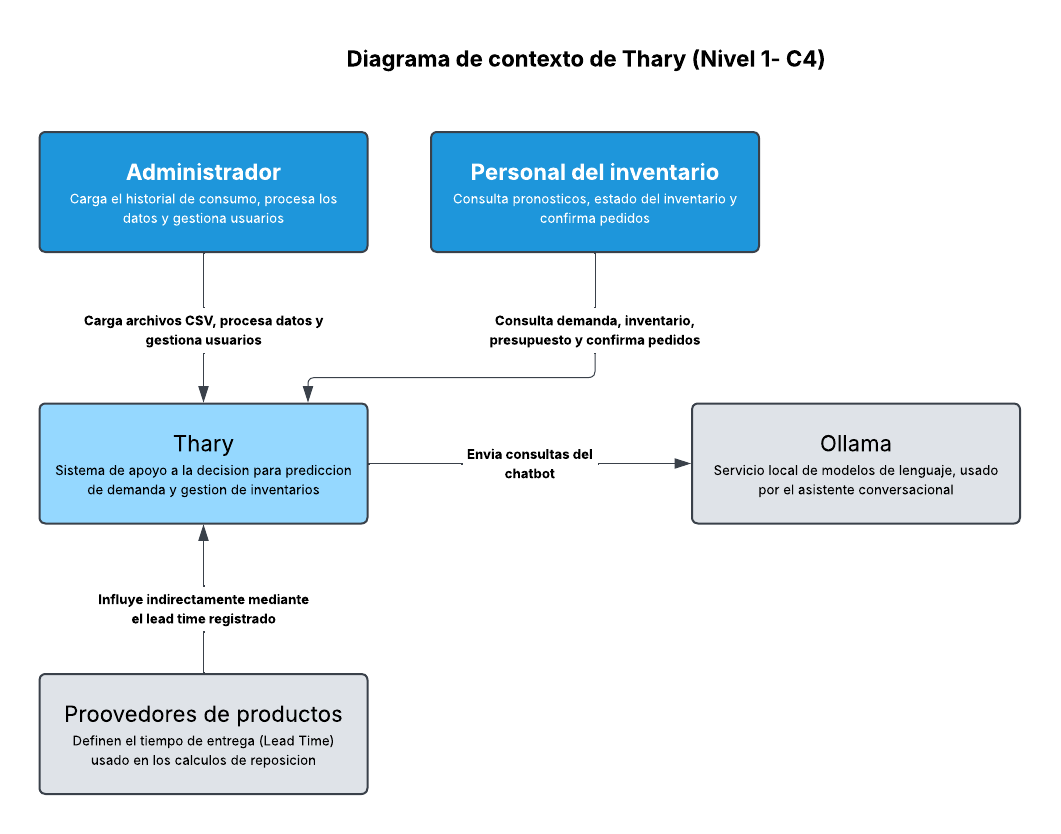
\includegraphics[width=0.7\textwidth]{templatefigures/Nivel1_Contexto}
    \caption{Diagrama de contexto del sistema (nivel 1 del modelo C4).}
    \label{fig:c4-contexto}
\end{figure}

Como se observa en la Fig. \ref{fig:c4-contexto}, el sistema interactúa con los actores identificados en la sección \ref{sec:stakeholders}.

\begin{figure}[H]
    \centering
    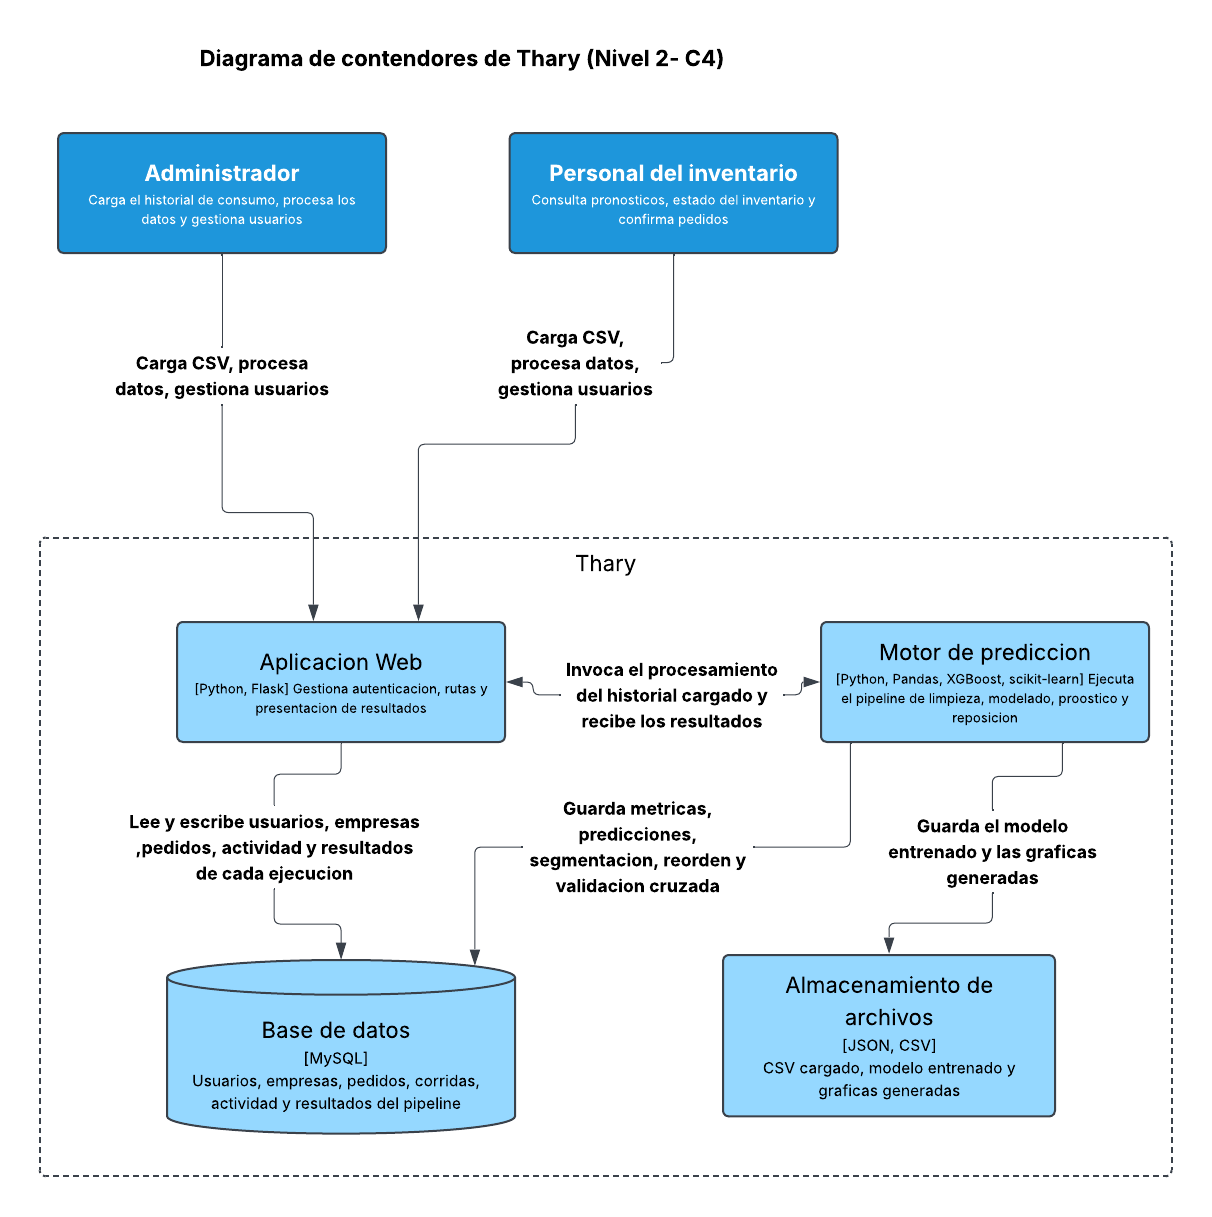
\includegraphics[width=0.7\textwidth]{templatefigures/Nivel2_Contenedores}
    \caption{Diagrama de contenedores del sistema (nivel 2 del modelo C4).}
    \label{fig:c4-contenedor}
\end{figure}

En la figura \ref{fig:c4-contenedor} se puede observar como se organizaron los contenedores del sistema Thary, factores como la aplicación web, el motor de predicción y la base de datos son contenedores independientes que se comunican entre si para el correcto funcionamiento del sistema. 

\begin{figure}[H]
    \centering
    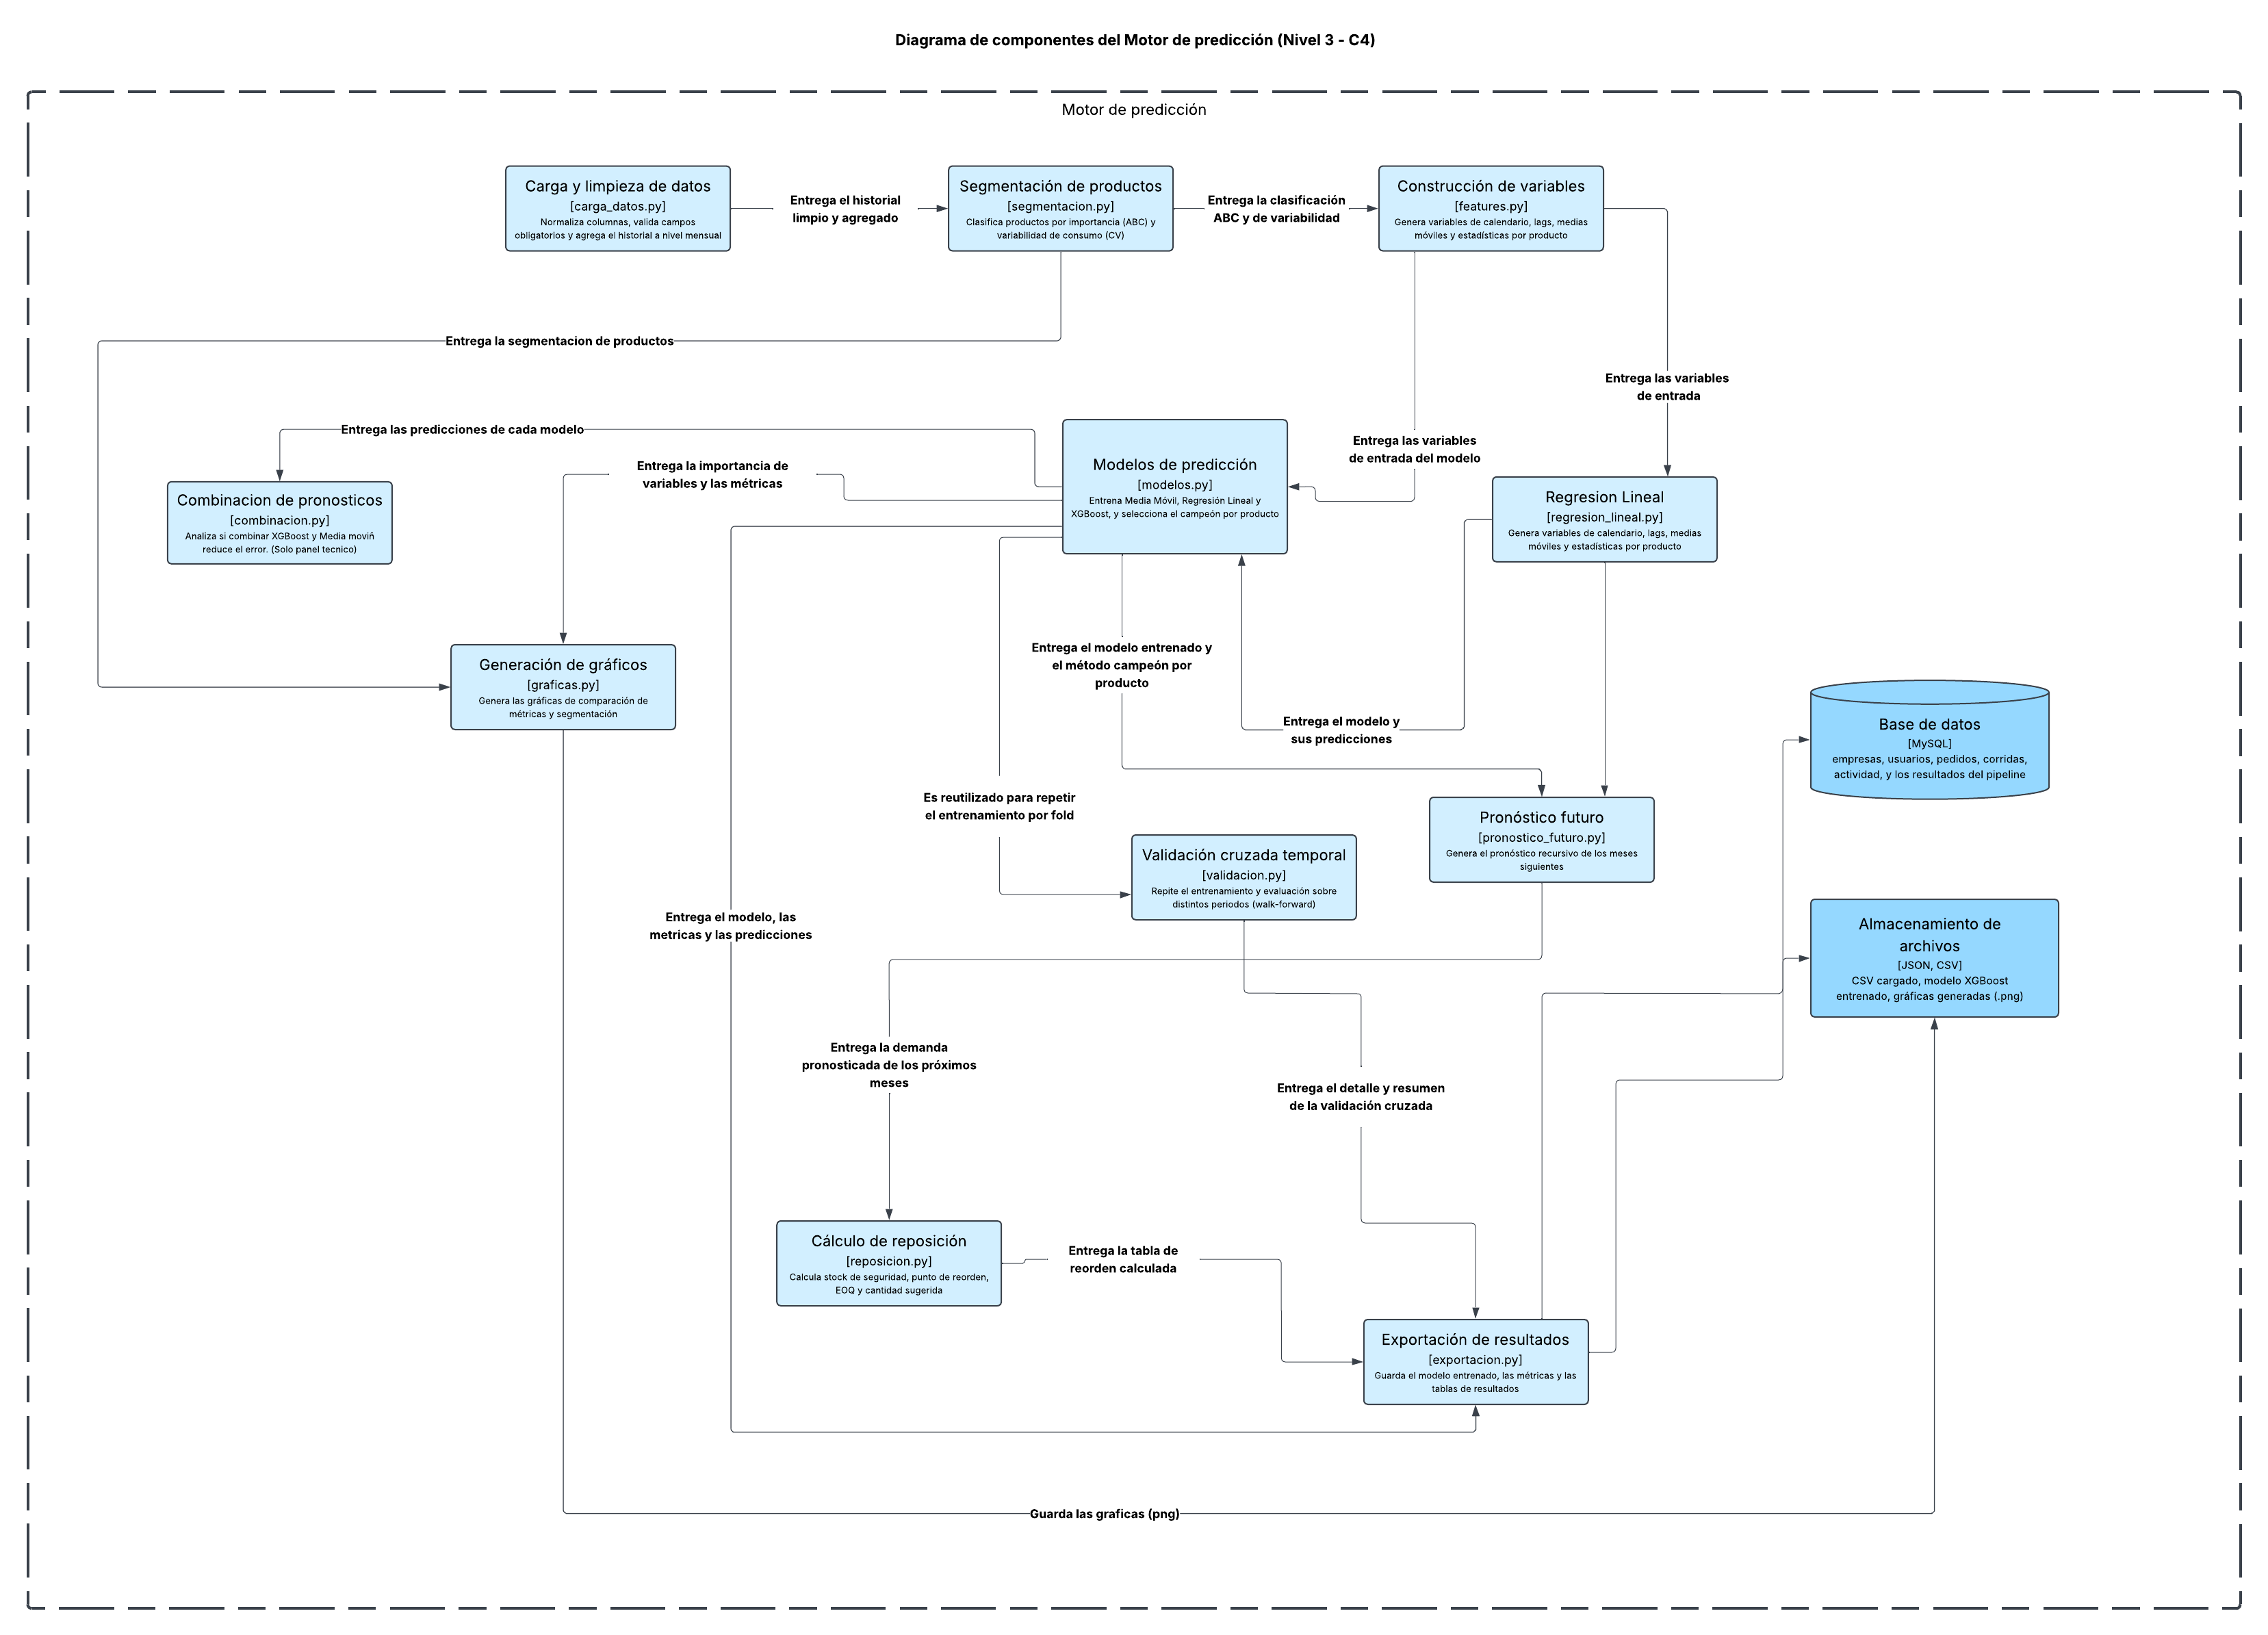
\includegraphics[width=0.7\textwidth]{templatefigures/Nivel3_Componentes}
    \caption{Diagrama de componentes del sistema (nivel 3 del modelo C4).}
    \label{fig:c4-componente}
\end{figure}

Finalmente, el diagrama de componentes detalla a profundidad el funcionamiento interno del motor de predicciones.
